%%%%%%%%%%%%%%%%%%%%%%%%%%%%%%%%%%%%%%%%%%%%%%
% Header
\documentclass[11pt]{report}
\usepackage[english]{babel}
\usepackage[utf8x]{inputenc}
\PassOptionsToPackage{hyphens}{url}\usepackage{hyperref}
\usepackage{graphicx}
\usepackage{fullpage}
\usepackage{nicefrac}
\usepackage[lastexercise]{exercise}
\usepackage[dvipsnames]{xcolor}
\usepackage{listings}

\setlength{\parindent}{0cm}

\renewcommand{\ExerciseHeader}{\large\textbf{\ExerciseName~\ExerciseHeaderNB} - \textbf{\ExerciseTitle}\medskip}

\renewcommand{\ExePartHeader}{\medskip\textbf{\ExePartName\ExePartHeaderNB\ExePartHeaderTitle\medskip}}

\begin{document}
%%%%%%%%%%%%%%%%%%%%%%%%%%%%%%%%%%%%%%%%%%%%%%
\title{Exercises -- Week 8: New Title}
\subsubsection*{EMAT10007 -- Introduction to Computer Programming}
\section*{\Large Exercises -- Week 8. Matplotlib}

Exercises this week will explore the use of Matplotlib, a python module designed for data visualisation.
\\
\textbf{Note:} The standard was to import the matplotlib module is by adding the following line at the start of your code: {\tt import matplotlib.pyplot as plt}. Any function belonging to the  matplotlib module can then be accessed by writing, for example, {\tt plt.plot()}.

\subsection*{\Large Part 1. Intro to MatPlotLib}
\begin{Exercise}[title= Line graph] \label{Ex:Variables}
	\Question{Create two lists of integers named {\tt x} and {\tt f} with the following values: \\
	{\tt x = [0,2,4,5,8,10]}\\
	{\tt y = [1,3,3,3,4,5,6]}\\
	Now try to plot these values using the {\tt plt.plot()} function. What error occurs? Can you guess why?}
	\Question{Try again with the following lists:\\
	{\tt x = [0,2,4,5,8,10]}\\
	{\tt y = [1,3,3,4,5,6]}\\
    \textbf {Hint:}	Remember to use {\tt plt.show()} to display the graph.}
	\Question{Now alter your graph so it has the following: 
	\begin{itemize}
	    \item x axis label: {\tt x}
	    \item y axis label: {\tt y}
	    \item title: {\tt Plot of y vs x}
	    \end{itemize}
	    }
	\Question{Finally, modify your code so the resulting graph looks like the graph in the following figure: \\
    
    \end{Exercise}
    	
    \begin{figure}[!h]
        \centering
        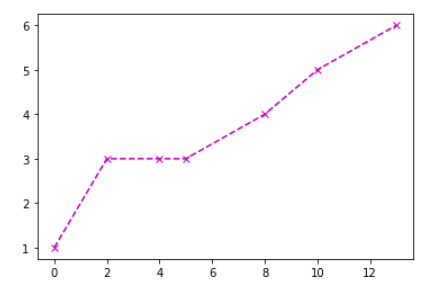
\includegraphics[height=5.5cm]{lineGraph.png}
        \caption{Final plot for Exercise 1.}
        \label{fig:lineGraph}
    \end{figure}
    
        \textbf{Hint:} Use the optional format string and {\tt plt.legend()} function as described in the lecture notes. You can look up detailed information on the {\tt plt.plot()} function here: \href{https://matplotlib.org/3.1.1/api/_as_gen/matplotlib.pyplot.plot.html}{\it{https://matplotlib.org/3.1.1/api/\_as\_gen/matplotlib.pyplot.plot.html}}, including details of the marker styles and colours that can be displayed in the optional format string.}


\subsection*{\Large Part 2. Saving plots and importing}

\begin{Exercise}[title= Histograms and csv] \label{Ex:Variables}
	\Question{Create a function named {\tt diceRolls} that prints out the results of a number {\tt n} of dice rolls. Make {\tt n} a variable that can be passed to the function. \\
	\textbf{Hint:} Use the numpy {\tt np.random.randint()} function.}
	\Question{Create a .csv file named {\tt diceRolls.csv} in the same folder as your code (you can do this using notepad, excel...).
	Modify the {\tt diceRolls} function so it saves the results in {\tt diceRolls.csv}.\\
	\textbf{Note:} Remember to add {\tt import csv} at the start of your code.\\
	\textbf{Hint:} Replace the {\tt <?>} in the following code with the result of the diceRolls function: \\
	{\tt with open('diceRolls.csv',mode='w') as f: }\\
	\hspace*{2em}{\tt writer = csv.writer(f, delimiter = ',')}\\
	\hspace*{2em}{\tt \tab writer.writerow(<?>) }}\\
	Run your code with {\tt n = 100} and check your {\tt diceRolls.csv} file to make sure data has been saved.  
    	}
	\Question{Now import the dice rolls from your diceRolls.csv file and save it as a numpy array named {\tt data} as described in the lecture slides. Print out the values of data to screen.}
	\Question{Let's try to visualise that data. First, try using {\tt plt.plot()}. This shows the results of each dice roll, but is slightly confusing to look at. }
	\Question{Now, let's try to represent the distribution of dice rolls using a histogram. Use {\tt plt.hist()} as described in the lectures and {\tt plt.show()} to visualise the histogram. }
	\Question{Add a title and x and y axis labels to your histogram. Try running your code with n = 10, 100, 1,000 and 10,000 to see how the distribution of dice rolls changes. }

\end{Exercise}


\subsection*{\Large Part 3. Curve fitting}

\begin{Exercise}[title= Polynomials] \label{Ex:Variables}
	\Question{Generate two random numpy arrays of 20 floats ranging from 1 to 10, named {\tt x} and {\tt y}. Sort the lists.\\
	\textbf{Hint:} Use {\tt np.random.uniform()} and {\tt np.sort()}.}
	\Question{Display the data from the sorted {\tt x} and {\tt y} functions using the {\tt plt.scatter()} function. }
	\Question{Use polyfit to determine the coefficients of a second degree polynomial ({\tt deg = 2}) fit to your {\tt x} and {\tt y} data. Then use {\tt poly1d} to generate a new array of fitted data, {\tt yfit}.}
	\Question{Show the original data using {\tt plt.scatter} and the fitted data using {\tt plt.plot()} in the same graph. Add a title, legend and x and y axis labels to the graph. }
	\Question{Modify your code so the polynomial fit is now of the 5th degree (set the 3rd parameter of {\tt polyfit} to 5). How doese this affect the fit to your data?}
\end{Exercise}


\end{document}